\documentclass[10pt,handout]{beamer}

\usetheme[progressbar=frametitle]{metropolis}
\usepackage{appendixnumberbeamer}

\usepackage{booktabs}
\usepackage[scale=2]{ccicons}

\usepackage{pgfplots}
\usepgfplotslibrary{dateplot}

\usepackage{xspace}
\newcommand{\themename}{\textbf{\textsc{metropolis}}\xspace}

\usepackage{listings}

\title{lmutils}
\subtitle{Tools for blazingly fast statistical analysis}
\date{}
\author{Josef Graf}
\institute{Department of Computing and Software, McMaster University}

\begin{document}

\maketitle

\begin{frame}{Table of contents}
  \setbeamertemplate{section in toc}[sections numbered]
  \tableofcontents%[hideallsubsections]
\end{frame}

\section[RARity Case Study]{RARity Case Study}

\begin{frame}{Context}
  \begin{itemize}[<+->]
    \item RARity uses a large multiple linear regression to calculate the $R^2$ value between a set of gene blocks and a set of phenotypes, finding the heritability of the phenotypes.
    \item The original code was written in \textbf{148 lines} of pure R,
      and by no fault of the original author (purely that of R) was slow.
    \item A single phenotype and gene block took
      \textbf{42 minutes and 38 seconds} to run.
    \item For a full UKB run this would take days, if not weeks.
  \end{itemize}
\end{frame}

\begin{frame}[fragile]{The Code}
\begin{verbatim}
lmutils::set_num_worker_threads(32)
phenos <- lmutils::Mat$new("phenos.rkyv")
phenos$remove_column("eid")
genos <- lmutils::Mat$new("genos.rkyv")
genos$min_column_sum(2)
genos$na_to_column_mean()
genos$standardize_columns()
genos$remove_column("eid")
df <- lmutils::calculate_r2(genos, phenos)
\end{verbatim}
  \begin{itemize}
    \item<2-> The new code is only \textbf{9 lines} long and makes
      use of a variety of functions from lmutils.
    \item<3-> A single phenotype and gene block can now be run in
      as little as \textbf{44 seconds}.
  \end{itemize}
\end{frame}

\begin{frame}[fragile]{What!?! But how!}
  \begin{itemize}[<+->]
    \item Parallelism
      \begin{itemize}
        \item Using 1 thread instead of 32 only adds about 4 and a half minutes.
      \end{itemize}
    \item rkyv
      \begin{itemize}
        \item Loading from \texttt{.RData} instead of \texttt{.rkyv} only adds about 10 seconds.
      \end{itemize}
    \item So where does the rest of the time go?
    \item Rust
    \item faer
      \begin{itemize}
        \item SIMD, parallelism, linear algebra magic.
      \end{itemize}
  \end{itemize}
\end{frame}

\section[Welcome to lmutils]{Welcome to lmutils}

\subsection{Getting Started}

\begin{frame}[fragile]{Installation}
  First, you need to install the Rust toolchain. You can do this by running
\begin{verbatim}
curl --proto '=https' --tlsv1.2 -sSf https://sh.rustup.rs | sh
\end{verbatim}
  Then, you can install lmutils by running the following in R. Once the package is in a more final state I'm going to submit it to CRAN.
\begin{small}
\begin{verbatim}
install.packages(
"https://github.com/GMELab/lmutils.r/archive/refs/heads/master.tar.gz",
repos=NULL) # use .zip for Windows
# OR
devtools::install_github("GMELab/lmutils.r")
\end{verbatim}
\end{small}
\end{frame}

\begin{frame}{Introductory definitions}
  \begin{itemize}[<+->]
    \item \textbf{Matrix-convertible object:} a data frame, matrix, file name, numeric column vector, or a \texttt{Mat} object.
    \item \textbf{List of matrix-convertible objects:} a list of matrix-convertible objects, a character vector of file names, or a single matrix-convertible object.
    \item \textbf{Standard output file:} a character vector or list of file names matching the length of the inputs or \texttt{NULL} to return the output. If a single input (not in a list) was given, the output will not be in a list.
    \item \textbf{Core parallelism:} the number of primary operations that will be run in parallel (i.e. gene blocks processed at once, files read at once, etc.).
  \end{itemize}
\end{frame}

\begin{frame}[fragile]{The \texttt{Mat} object}
  \begin{itemize}[<+->]
    \item The \texttt{Mat} object is a wrapper around lmutils's internal representation of a matrix.
    \item It allows for easy, efficient, and lazy manipulation of the matrix.
    \item It is the recommended way to interact with the newest version of lmutils.
  \end{itemize}
\begin{verbatim}
mat <- lmutils::Mat$new("phenos.rkyv")
eids <- mat$col("eid")
r <- mat$r() # just like any other R matrix
colnames(r) == mat$colnames() # TRUE
r$eid == eids # TRUE
\end{verbatim}
\end{frame}

\subsection{Working with Files}

\begin{frame}[fragile]{File Types}
  lmutils supports a variety of both compressed and uncompressed file formats.
  \begin{itemize}
    \item \texttt{.csv} (\texttt{.csv.gz}) comma-separated values, first row is the column header.
    \item \texttt{.tsv} (\texttt{.tsv.gz}) tab-separated values, first row is the column header.
    \item \texttt{.txt} (\texttt{.txt.gz}) space-separated values, first row is the column header.
    \item \texttt{.rkyv} (\texttt{.rkyv.gz}) a binary format that is both fast and space-efficient (\textbf{recommended}).
    \item \texttt{.RData} an R-specific binary format.
  \end{itemize}
\end{frame}

\begin{frame}[fragile]{Reading and Writing Files}
  lmutils supports two methods of reading and writing files, using the \texttt{Mat} object or global functions.
  \begin{verbatim}
mat <- lmutils::Mat$new("phenos.rkyv")
r <- mat$r()
mat$save("phenos.csv")

# both functions support a list of files
lmutils::load("phenos.rkyv")
lmutils::save(
    list("file1.csv", matrix(1:9, nrow=3), 1:3,
      data.frame(a=1:3, b=4:6), mat),
    c("file1.tsv", "file2.rkyv.gz", "file3.rkyv",
      "file4.rdata", "file5.tx.gz")),
)
\end{verbatim}
\end{frame}

\subsection{Configuration}

\begin{frame}{Configuration}
  lmutils provides a number of global configuration options that can be set using environment variables or through various functions. Please note, these generally cannot be changed after calling any other lmutils functions.
  \begin{itemize}[<+->]
    \item \texttt{LMUTILS\_LOG} / \texttt{lmutils::set\_log\_level}: the log level, defaults to \texttt{info}. The valid levels (in order of increasing verbosity) are \texttt{off}, \texttt{error}, \texttt{warn}, \texttt{info}, \texttt{debug}, and \texttt{trace}.
    \item \texttt{LMUTILS\_CORE\_PARALLELISM} / \texttt{lmutils::set\_core\_parallelism}: the number of primary operations that will be run in parallel, defaults to 16.
    \item \texttt{LMUTILS\_NUM\_WORKER\_THREADS} / \texttt{lmutils::set\_num\_worker\_threads}: the number of worker threads, defaults to \texttt{num\_cpus / 2}.
    \item \texttt{LMUTILS\_ENABLE\_PREDICTED} / \texttt{lmutils::disable\_predicted} / \texttt{lmutils::enable\_predicted}: whether to calculate and return predicted values in linear models, defaults to disabled for performance reasons.
  \end{itemize}
\end{frame}

\subsection{Matrix Manipulation}

\begin{frame}{Matrix Manipulation}
  lmutils provides more than 30 functions just for manipulating \texttt{Mat} objects, not to mention more than a dozen other global functions for matrices and data frames. Here are a few examples.
  \begin{itemize}[<+->]
    \item \texttt{Mat\$remove\_column(col)}: remove a column by name.
    \item \texttt{Mat\$min\_column\_sum(threshold)}: remove columns with a sum below a threshold.
    \item \texttt{Mat\$na\_to\_column\_mean()}: replace \texttt{NA} values with the column mean.
    \item \texttt{Mat\$standardize\_columns()}: standardize columns to have a mean of 0 and a standard deviation of 1.
    \item \texttt{Mat\$transpose()}: transpose the matrix.
    \item \texttt{Mat\$sort(col\_idx)}: sort the matrix by a column.
    \item \texttt{Mat\$dedup(col\_idx)}: deduplicate the matrix by a column.
  \end{itemize}
  A full list of functions can be found in the documentation on GitHub at \hyperlink{https://github.com/GMELab/lmutils.r}{github.com/GMELab/lmutils.r}.
\end{frame}

\subsection{Statistical Functions}
\begin{frame}{Statistical Functions}
  lmutils also provides a number of lightning fast statistical functions.
  \begin{itemize}[<+->]
    \item \texttt{lmutils::compute\_r2(v1, v2)}: compute the $R^2$ between two vectors.
    \item \texttt{lmutils::mean(v)}: compute the mean of a vector.
    \item \texttt{lmutils::median(v)}: compute the median of a vector.
    \item \texttt{lmutils::sd(v)}: compute the standard deviation of a vector.
    \item \texttt{lmutils::var(v)}: compute the variance of a vector.
  \end{itemize}
\end{frame}

\subsection{Analysis Functions}

\begin{frame}[fragile]{\texttt{calculate\_r2}}
  The first kind of primary analysis is calculating the $R^2$ value between a list of matrix convertible objects (i.e. gene blocks) and a single matrix convertible object (i.e. phenotypes).
\begin{verbatim}
df <- lmutils::calculate_r2(list("genos1.rkyv", "genos2.rkyv",
"genos3.rkyv"), "phenos.rkyv")
\end{verbatim}
  \pause
  The output is a data frame with the columns:
  \begin{itemize}[<+->]
    \item \texttt{r2}: the $R^2$ value.
    \item \texttt{adj\_r2}: the adjusted $R^2$ value.
    \item \texttt{data}: the name or index of the data.
    \item \texttt{outcome}: the name or index of the outcome.
    \item \texttt{n}: the number of samples, i.e. rows.
    \item \texttt{m}: the number of predictors, i.e. SNPs.
    \item \texttt{predicted}: the predicted values of the outcome for each sample, only returned if enabled.
  \end{itemize}
\end{frame}

\begin{frame}[fragile]{\texttt{column\_p\_values}}
  The second kind of primary analysis is calculating the $p$-values of each pair of data and outcome columns. In some testing it can do a 20 thousand column block in about 2-3 seconds.
  \begin{verbatim}
df <- lmutils::column_p_values(list("genos1.rkyv",
"genos2.rkyv", "genos3.rkyv"), "phenos.rkyv")
\end{verbatim}
  \pause
  The output is a data frame with the columns:
  \begin{itemize}[<+->]
    \item \texttt{p\_value}: the $p$-value of the regression.
    \item \texttt{beta}: the slope of the regression.
    \item \texttt{intercept}: the intercept of the regression.
    \item \texttt{data}: the name or index of the data.
    \item \texttt{data\_column}: the index of the column in the data.
    \item \texttt{outcome}: the name or index of the outcome.
  \end{itemize}
\end{frame}

\section{plots.r}

\begin{frame}[fragile]{plots.r}
  \begin{itemize}[<+->]
    \item \texttt{plots.r} is a small package for creating publication-ready plots.
    \item It currently only supports forest plots thanks to \texttt{metafor}, but I'm happy to add more upon request!
  \end{itemize}
  \pause
  It can be installed by running the following in R.
  \begin{small}
  \begin{verbatim}
install.packages(
"https://github.com/GMELab/plots.r/archive/refs/heads/master.tar.gz",
repos=NULL) # use .zip for Windows
# OR
devtools::install_github("GMELab/plots.r")
\end{verbatim}
\end{small}
\end{frame}

\begin{frame}[fragile]{Basic Forest Plot}
  \begin{verbatim}
plots.r::basic_forest_plot(
    x = c(0.1, 0.2, 0.3, 0.4, 0.5),
    se = c(0.01, 0.02, 0.03, 0.04, 0.05),
    width = 500,
    height = 300,
    name = "Example",
    header = c("Left", "Right"),
    slab = c("Study 1", "Study 2", "Study 3",
             "Study 4", "Study 5"),
    xlab = "X-axis label",
)
\end{verbatim}
\end{frame}

\begin{frame}{Basic Forest Plot}
  \begin{center}
    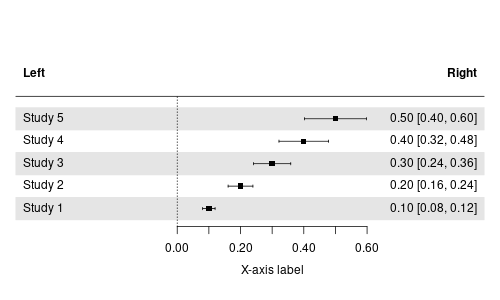
\includegraphics[width=0.8\textwidth]{Example.png}
  \end{center}
\end{frame}

\begin{frame}[fragile]{Grouped Forest Plot}
  \begin{verbatim}
plots.r::grouped_forest_plot(
    x = list(c(0.1, 0.2, 0.3, 0.4, 0.5),
             c(0.1, 0.2, 0.3, 0.4, 0.5)),
    se = list(c(0.01, 0.02, 0.03, 0.04, 0.05),
              c(0.01, 0.02, 0.03, 0.04, 0.05)),
    width = 500,
    height = 500,
    name = "Grouped_Example",
    header = c("Left", "Right"),
    slab = c("Study 1", "Study 2", "Study 3",
             "Study 4", "Study 5"),
    xlab = "X-axis label",
    glab = c("Group 1", "Group 2"),
)
\end{verbatim}
\end{frame}

\begin{frame}{Grouped Forest Plot}
  \begin{center}
    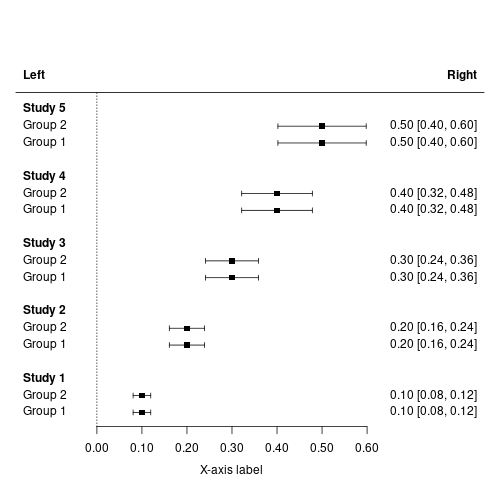
\includegraphics[width=0.7\textwidth]{Grouped_Example.png}
  \end{center}
\end{frame}

\section[Conclusion]{Conclusion}

\begin{frame}{Conclusion}
  \begin{itemize}
    \item<1-> Thank you for listening!
    \item<2-> Feel free to ask me questions anytime, I'm always happy to help or add new things. :)
    \item<2-> \hyperlink{mailto:grafj1@mcmaster.ca}{\textbf{grafj1@mcmaster.ca}} or \textbf{Josef Graf} on Teams.
    \item<3-> The presentation is available at \hyperlink{https://github.com/mrvillage/lmutils-presentation}{github.com/mrvillage/lmutils-presentation}.
    \item<3-> More information on lmutils can be found at \hyperlink{https://github.com/GMELab/lmutils.r}{github.com/GMELab/lmutils.r}.
    \item<3-> More information on plots.r can be found at \hyperlink{https://github.com/GMELab/plots.r}{github.com/GMELab/plots.r}.
  \end{itemize}
\end{frame}

\end{document}
